\input{../header}
\hyphenpenalty=5000

\rhead{Your name: \rule{8cm}{0.15mm}}

\begin{document}

\everymath{\displaystyle}

\section{Learning target D2, version 1}

D2: Express real world situations as differential equations, determine any equilibrium solutions, and explain the significance of the equilibrium solutions in context.

\hrulefill

A population of flamingos changes over time according to the differential equation 
\[\dfrac{dP}{dt} = -\frac{1}{3}\, P\, (1-P)(5-P),\]
where $P$ is measured in thousands (and $t$ is probably measured in months or years).

Draw a phase graph and a slope field. Find all the equilibrium solutions, and explain how you know each one is stable or unstable.
 
\begin{center}
	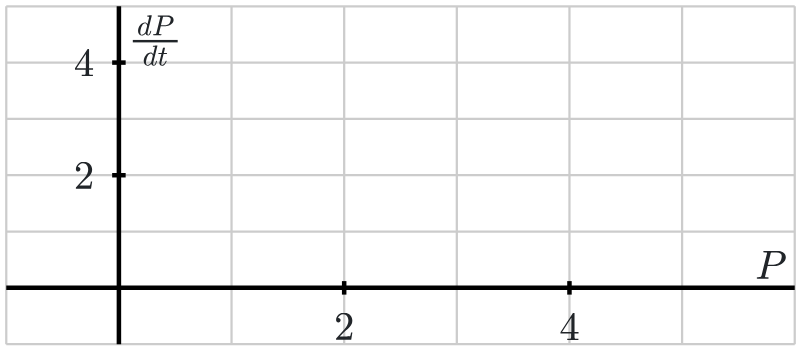
\includegraphics[width=0.75\textwidth]{../images/d2-phase-graph-axes.png}

	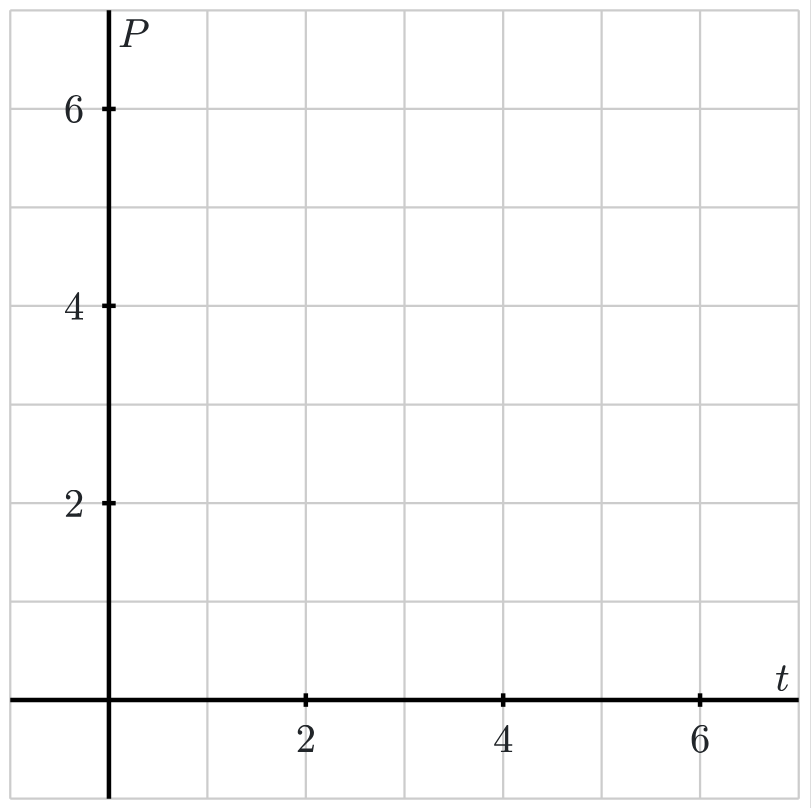
\includegraphics[width=0.7\textwidth]{../images/d2-slope-field.png}
\end{center}
\pagebreak

\section{Learning target D3, version 1}

D3: Apply Euler's Method to generate an approximate solution to an initial value problem, and explain the result's meaning in context.

\hrulefill

A population of flamingos changes over time according to the differential equation 
\[\dfrac{dP}{dt} = -\frac{1}{3}\, P\, (1-P)(5-P),\]
where $P$ is measured in thousands (and $t$ is probably measured in months or years).

\begin{enumerate}[(a), leftmargin=0pt]
	\item If $P(0) = 0.5$, use Euler's method with 3 steps to approximate $P(2)$. Record your work in a table.\\
	(Hint: If you're using 3 steps to get from $t=0$ to $t=2$, how big should $\Delta t$ be?)
	\vfill
	\item Same thing, but this time, start with $P(0) = 1.5$.
	\vfill
	\item Compare your numerical results here with your graphical results on the D2 part of this problem. What recommendations do you have for flamingo keepers?
\end{enumerate}

%%%%%%%%%%%%%%%%%%%%%%%%%%%%%%%%%%%%%%%%%%%%%%%%%%%%%%%
%\pagebreak
%%%%%%%%%%%%%%%%%%%%%%%%%%%%%%%%%%%%%%%%%%%%%%%%%%%%%%%

\end{document}